\chapter{Introducción}

Actualmente las aplicaciones web prestan servicios de forma totalmente gratuita a cambio de los datos que recopilan de los usuarios. En la mayoría de casos esta información se rentabiliza a través de servicios de marketing y publicidad que desean vender un producto o servicio determinado. Por ello, estos servicios necesitan perfilar al usuario en cuestión para así ofrecerle un producto que les pueda interesar.\par
La técnica de seguimiento más conocida  son las \textit{cookies}, las cuales se almacenan en el propio dispositivo y que luego son usadas para uso estadístico y para mejorar la experiencia del usuario.\par
Algunos exploradores permiten deshabilitar su uso y ciertos antivirus realizan borrados periódicos de los ficheros de rastreo, pero la mayoría de aplicaciones web no dejan acceder a sus servicios, o la totalidad de los mismos, si no permiten su uso.\par
La huella digital ofrece una fuente de información sobre un determinado dispositivo con la finalidad de identificarlo, singularizarlo, y hacer un seguimiento con el propósito de perfilarlo.\par
Ese conjunto de datos permite prácticamente, de forma unívoca, identificar dicho terminal y en cuestión a la persona o grupo de personas que puedan estar usándolo. Por lo general, los terminales como los teléfonos móviles, tabletas, portátiles y ordenadores de sobremesa, son usados por una sola persona. Y por ello, podemos asumir que los datos recopilados de cierto dispositivo pertenecen a una persona en concreto.\par
Las entidades usan estos mecanismos de recopilación de datos con todos los terminales que se conecten a sus servidores, para así poder hacer un seguimiento del usuario y elaborar un perfil.\par
El desarrollo software de JavaScript, Flash y Microsoft Silverlight, facilitan la implementación de métodos para recoger información muy concreta del dispositivo, como es el tamaño de la pantalla o la versión del sistema operativo. La combinación de estas características permite perfilar al usuario e identificarlo.\par
Para el uso de las \textit{cookies} es común encontrar cláusulas de privacidad que permiten al usuario dar o no su consentimiento para el uso de éstas. Las técnicas de huella digital no requieren de autorización para que sean usadas. Así se consigue que, en el caso de que las primeras sean eliminadas, no se pierda la trazabilidad sobre el usuario y que éste, además, no pueda tomar medidas para evitarlo.\par

\section{Objetivos}
 
El principal objetivo de este proyecto es crear una aplicación web que permita recopilar los datos de un terminal, aplicando las distintas técnicas de \textit{fingerprinting}, y elaborar un perfil en base a ellos. En concreto tenemos las siguientes metas:
\begin{itemize}
    \item Crear una aplicación escalable, para que en el futuro se pueda continuar desarrollando según se requiera.
    \item Investigar la variedad de métodos de huella digital e implementarlos.
    \item Almacenamiento de datos, de los cuales se harán un perfilado y se guardarán en una base de datos.
\end{itemize}

\section{Plan de trabajo}
Para la planificación del proyecto hemos seguido una metodología clásica, en cascada, de tal modo que analizamos la extensión y profundidad y, en función de eso, distribuimos el tiempo que determinamos para cada tarea.\par
En el siguiente \textit{Diagrama de Gantt} se puede observar cómo ha sido el desarrollo. Tras la ampliación de los plazos de entrega, se actualizaron las tareas posteriores y sus respectivos tiempos.\par
\begin{figure}[H]
    \centering
    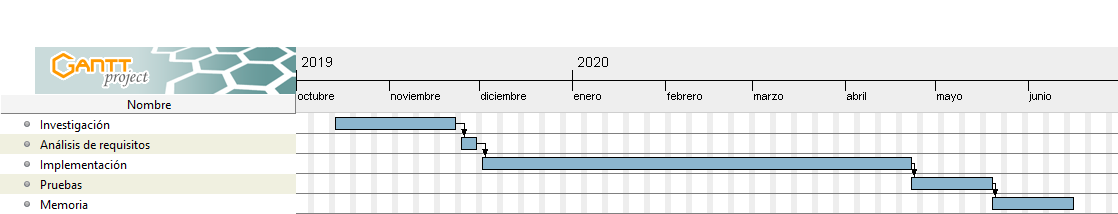
\includegraphics[width=1\textwidth]{Images/diagramaGantt.png}
    \caption{diagrama de Gantt}
    \label{fig:diagramaGantt}
\end{figure}